\documentclass[conference]{IEEEtran}
\IEEEoverridecommandlockouts
% The preceding line is only needed to identify funding in the first footnote. If that is unneeded, please comment it out.
\usepackage{cite}
\usepackage{amsmath,amssymb,amsfonts}
\usepackage{algorithmic}
\usepackage{float}
\usepackage{graphicx}
% \usepackage{longtable}
\usepackage{textcomp}
\usepackage{xcolor}
\def\BibTeX{{\rm B\kern-.05em{\sc i\kern-.025em b}\kern-.08em
    T\kern-.1667em\lower.7ex\hbox{E}\kern-.125emX}}
\begin{document}

\title{Simple Driving-Skill Evaluation System\\
{\footnotesize \textsuperscript
\\
}
\thanks{Identify applicable funding agency here. If none, delete this.}
}

\author{\IEEEauthorblockN{1\textsuperscript{st} Yuan-Pu Hsu}
\IEEEauthorblockA{\textit{Bourns.University of California,Riverside} \\
\textit{name of organization (of Aff.)}\\
Riverside, the United States \\
email address}
\and
\IEEEauthorblockN{2\textsuperscript{nd} Tianxiang Sun}
\IEEEauthorblockA{\textit{Bourns.University of California,Riverside} \\
\textit{name of organization (of Aff.)}\\
Riverside,the United States \\
email address}
\and
\IEEEauthorblockN{3\textsuperscript{rd} Given Name Surname}
\IEEEauthorblockA{\textit{dept. name of organization (of Aff.)} \\
\textit{name of organization (of Aff.)}\\
City, Country \\
email address}
\and
\IEEEauthorblockN{4\textsuperscript{th} Given Name Surname}
\IEEEauthorblockA{\textit{dept. name of organization (of Aff.)} \\
\textit{name of organization (of Aff.)}\\
City, Country \\
email address}
\and
\IEEEauthorblockN{5\textsuperscript{th} Given Name Surname}
\IEEEauthorblockA{\textit{dept. name of organization (of Aff.)} \\
\textit{name of organization (of Aff.)}\\
City, Country \\
email address}
\and
\IEEEauthorblockN{6\textsuperscript{th} Given Name Surname}
\IEEEauthorblockA{\textit{dept. name of organization (of Aff.)} \\
\textit{name of organization (of Aff.)}\\
City, Country \\
email address}
}

\maketitle

\begin{abstract}
Driving has became a indispensable part of American's daily life for decades.It gives us a lot of convenience. Meanwhile, unskillful driving could cause serious damage, not only for drivers but also for the society. Therefore, a driving skill evaluation system would be a hotpoint nowadays. 

In our project, we implement a simple driving-skill evaluation system, which can be put behind the windscreen of the car and recognizing patterns showing up on the road. By doing comparison between the pattern we get with the speed of the car, we do some evaluation about the driving skill of the driver. We build our own  iOS app to implement our system on. Besides, we constructed multiple Convolutional Neural Network(CNN) models to recognize traffic signs and traffic lights and achieving 99.8\% test accuracy for recognizing images taken in South California. Last but not least, we use php to connect our app with different platforms,like google cloud and PC.
\end{abstract}

\begin{IEEEkeywords}
Driving-skill evalution, Convolutional Neural Network(CNN),  Google cloud, PHP
\end{IEEEkeywords}

\section{Introduction}
Nowadays, over 90\% of families in the United States at least have one vehicle. Driving has already been a big portion of American's daily life for decades.Therefore, we want to make a simple system to evaluate the driving skill of drivers after finish a tour, and the only thing needed is a smart phone. We believe it could help drivers to evaluate their driving skill and improve their skill to some extent. Further, insurance company can also take advantage of this system to evaluate the credit of their clients by using their scores, while those who has higher scores, which means better driving skill could be benefit with lower insurance payment.

When it comes into detail, firstly we build an application on our mobile device(in our case, iPhone 6s) and use it to implement our system on. The user would be asked to put the phone behind the windscreen, and the application would automatically capture images of front view to recognize different kinds of patterns on the road. In our project, the recognized pattern has been restricted to traffic signs and traffic light. Additionally, in order to recognize patterns, we implement two different kinds of Convolutional Neural Networks (CNN). The first one is a VGGNet model, however, we find that the training time and running time would exceed one second, which would not fit our scenario. Therefore, we propose another 6-layers CNN network, which consisted by 6 convolutional layers, 3 max-pooling layers, 3 drop-out layers and a fully connected layer with softmax.The test accuracy of our model for GTBSRB is 96.4\%. Beside, by using Lisa dataset, test accuracy of traffic signs is 99.8\% and it is 99.5\% for traffic light. What is more, we implement our model on three different kinds platforms, iphone, google cloud and local terminal.  We calculate the data transfer time, CNN model running time and server running time (if they have)for those three platforms, respectively. The result


The contribution of our project is shown as follows: 

\textbullet We design our own iOS application by Swift deploying on iOS 11.2. In addition, we are able to measure the speed and acceleration, and compare with the recognized traffic sign and traffic light from road image in nearly real-time 

\textbullet We propose and construct our own CNN architecture which is a 6-layers CNN with 3 max-pooling layers, 3 drop-out layers and 1 fully-connected layer with softmax to conclude the results. The model is trained by using GTSRB and Lisa dataset for different kinds of scenarios.

\textbullet We evaluate the performance of our model. The result shows that our model can reach at least 96.4\% test accuracy with GTRSRB dataset, 99.5\% test accuracy for traffic lights and 99.8\% for traffic signs with LISA dataset.

\textbullet We implement three platforms to run our model on. We do some evaluation about the GPU we can used in google cloud. Besides, the models developed with the environment of Keras and Teensorflow are both deployed and tested on mobile device, local PC and Google cloud. 

\textbullet We use php to link our app with other platforms. It make us can transfer images which get by the app to other platforms and let they run the model to evaluate the running time for our model on different platforms. 


\section{Background and Related Work}

\subsection{Background}

\subsubsection{Convolutional Neural Network}

\

\noindent
Convolutional Neural Network(CNN) is a important, widely-used model in machine learning. It is a class of deep, feed-forward artificial neural networks, most commonly applied to analyzing visual imagery. 

Before going to the layer-level analysis, it is important to understand different kinds of layers used by our CNN model. 

Convolutional layers apply a convolution operation to the input and pass it to the output. By doing convolution between original image and filters, more detailed information are gotten and a feature map has been created.

Max-pooling layer is used to reshape the image by using the maximum value from each of the cluster of neurons at the prior layer.

Drop-out layer is a regularization technique to drop out some units in a neural network to reduce overfit in neural network.

Fully connected layer with softmax is used to flatten the result we gotten before. What is more, softmax can be using as the classifier to get the classification of the network.


\subsubsection{Tensorflow and Keras}

\

\noindent

Tensorflow, is an open source soeftware libaray for high performance numerical computation. Its flexible architecture allows easy deployment of computation acrosss a variety of platforms, and from desktop to clusters of serves to mobile and edge devices. In machine learning and deep learning, it does strong support and has been widely used.

Keras is a high-level neural networks API, written in Python and capable running on top of Tensorflow,CNTK, or Theano. It is much easier to easy use to deploy own neural network. Furthermore, it can decrease the running time significantly, which makes fast experimentation enable. 

\subsection{Related Work}

Before we began our work,we had been inspired by the work of Kang,Y.P. et al. [1]. In their paper, they did partitions for the neural network and running various parts on different platforms. Besides, Kang and his team evaluated the latency and energy consumption of their new system, which showed that their new system can achieve up to $40.7 \times$ latency speed-up, reduce mobile energy consumption by up to $94.7 \%$, and improve data-center throughput by up to $6.7 \times$. Additionally, we also got some inspired by the work of Shustanov, A. et al. [2] and Habibi Aghdam, H., et al [3]. while constructing our CNN model. In the work of former one, the team descirbe a revised end to end technology for detecting and recognizing traffic sign in real-time by CNN. It could use the speed received from the vehicle to predict not only the presence of the object but also the scale and its exact coordinates in the neighboring frame. In the latter work, the team proposed a light CNN which is designed for detecting traffic sign on high-resolution images. They trained the network in two steps. First, the negative sample would be randomly selected from the training image. Second, it has been used to train the CNN using more appropriate data. The result of prediction has increased to 99.89\% on GTSRB dataset. Besides, we learned from the work of Simonyan, K., et al.[4] about how to increase the performance while meeting a large-scale image recognition setting. The team showed in the paper that they designed an architecture which increased the depth of the CNN model. Their model showed only 6.8\% test error on top-5 testing.   



\section{System Model}

\begin{figure}[H]
\centering
  \begin{minipage}{.4\textwidth}
    \centering
    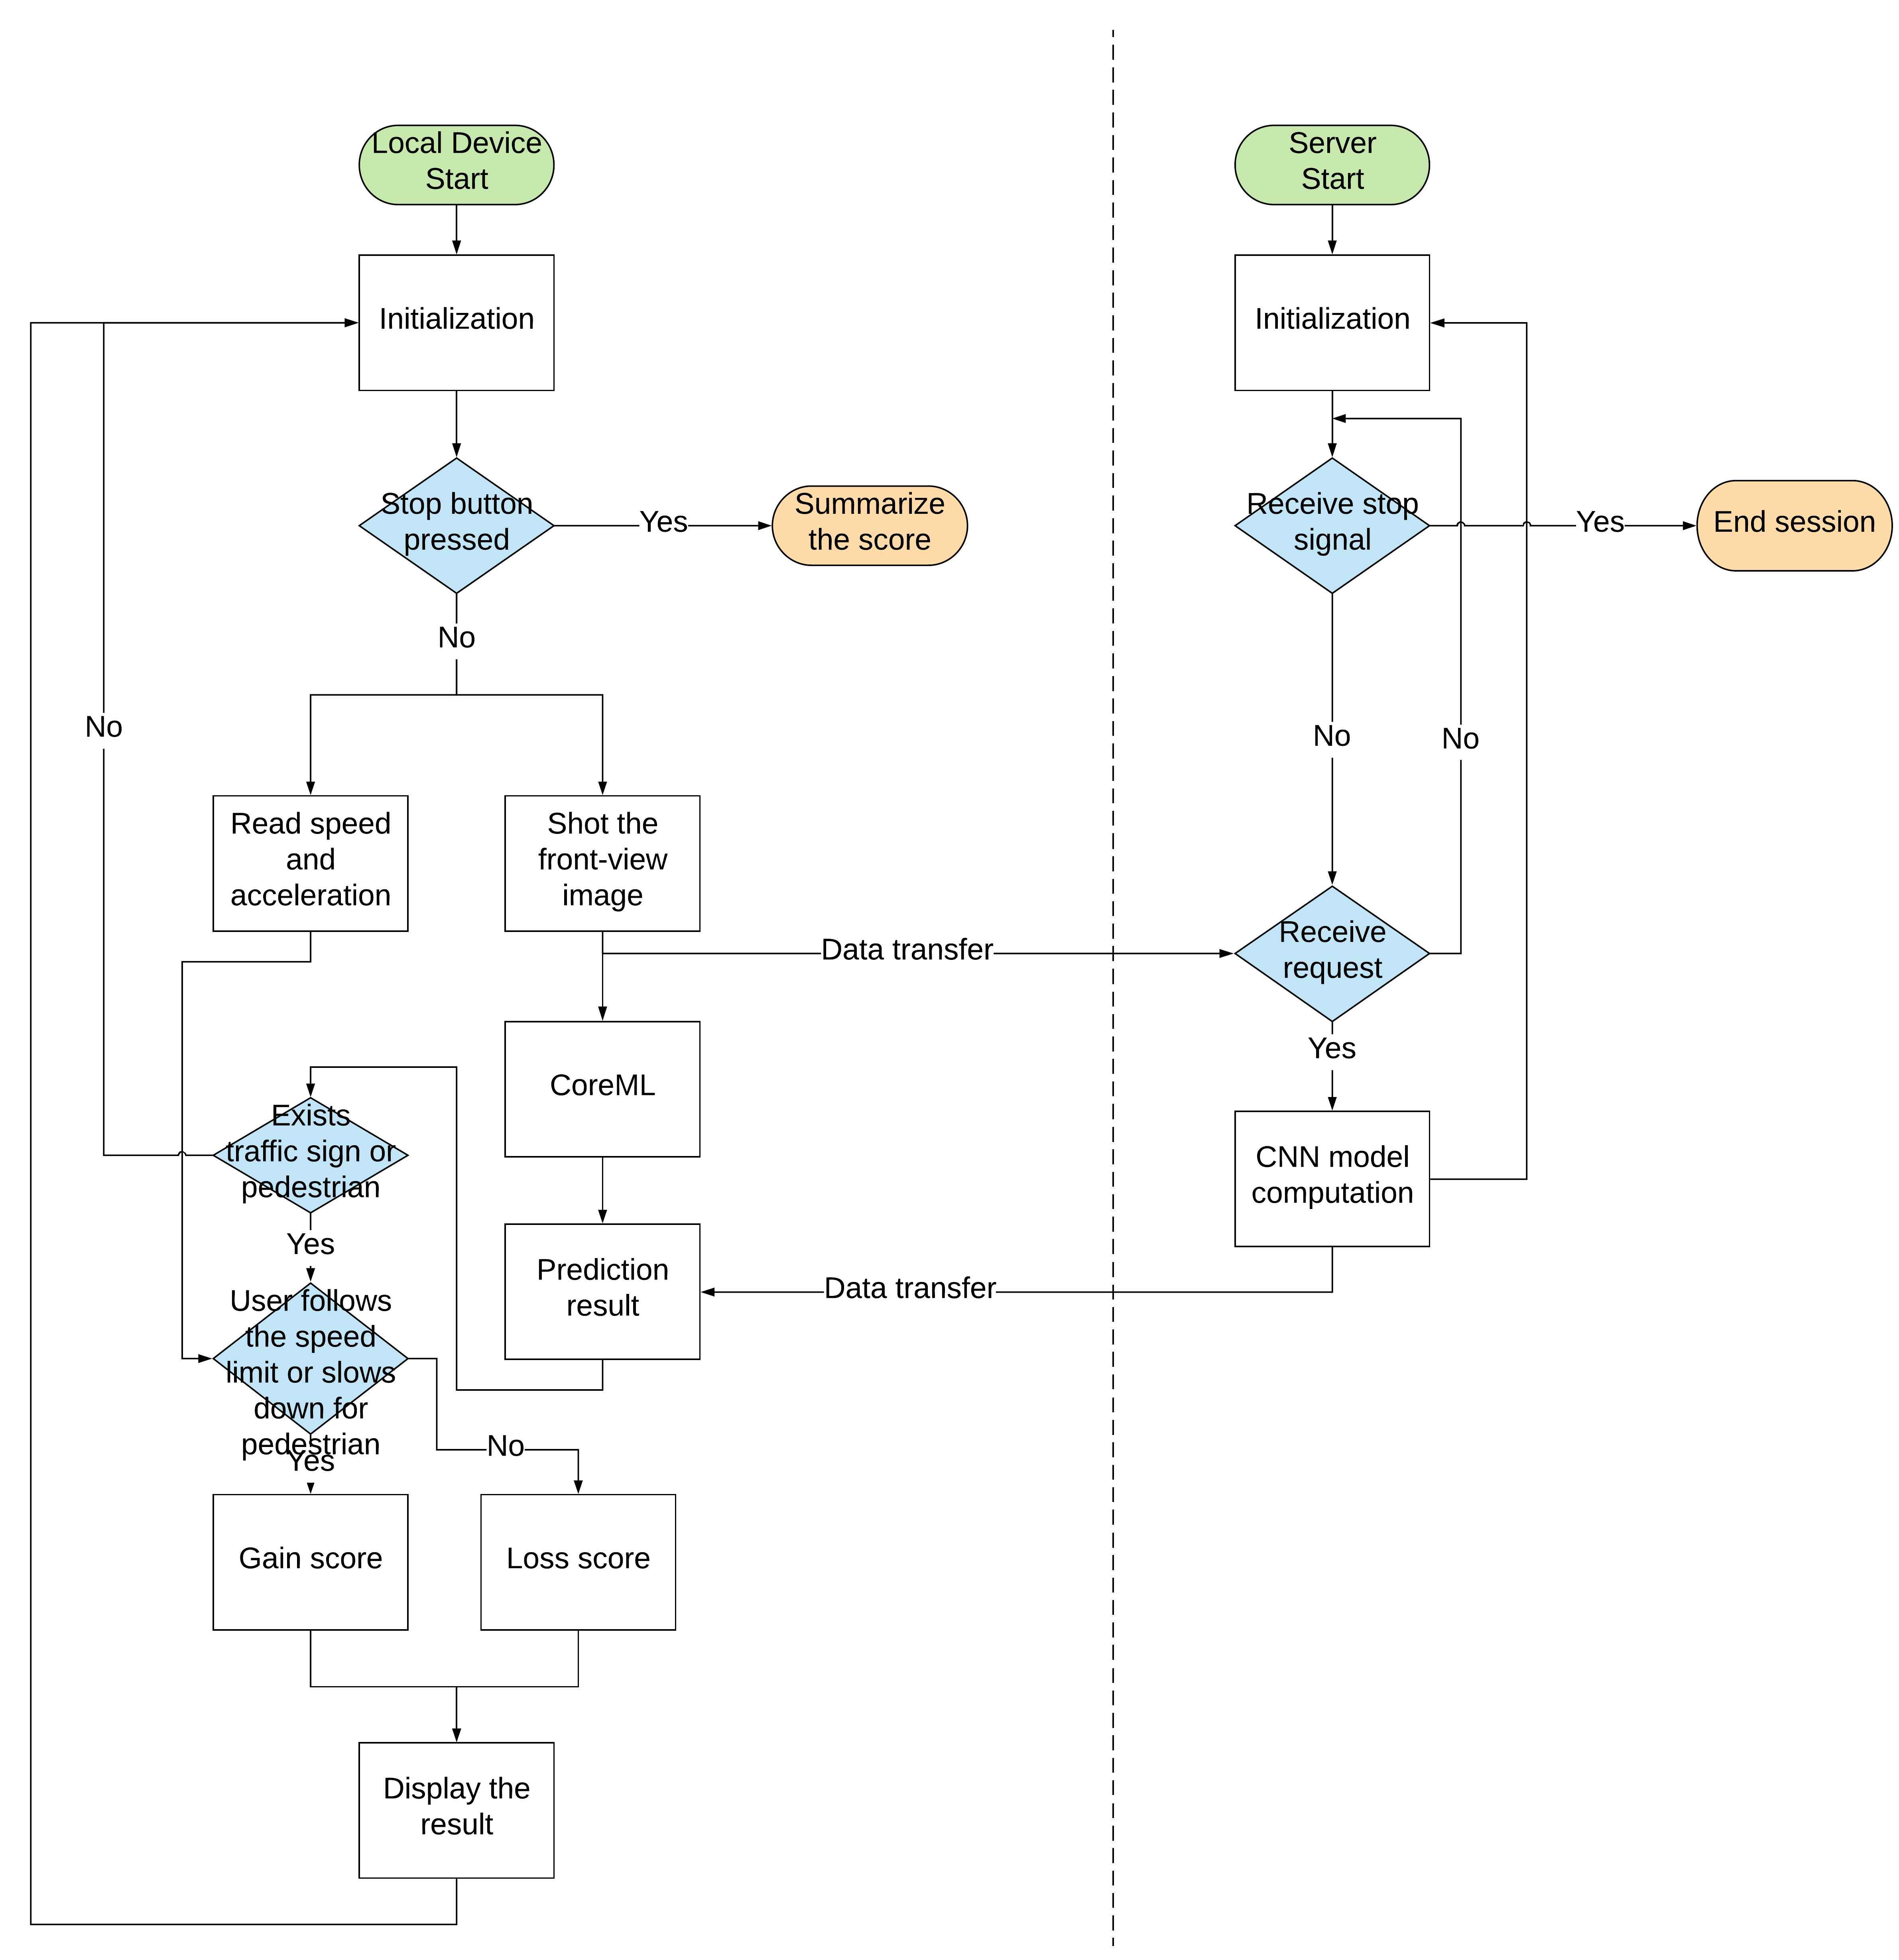
\includegraphics[width=1.2\linewidth]{system_flowchart.png}
    \caption{System Model Flowchart}
    \label{fig:fig_1}
  \end{minipage}
\end{figure}

Our proposed system model flowchart is shown above. 
\section{Proposed Work}
\subsection{iOS app Design}

We first build a simple application for taking the front-view images periodically, and record both the speed and acceleration at the same time via GPS and accelerometer. The picture will then pass through the trained CNN model installed in the bundle,or upload to the cloud service for the prediction. The result includes whether there existed a traffic sign or traffic light in the image, and what kind of sign it is. After the translation of the speed limit is done, the application can determine if the user was over speed or not. In the end, the application would give the user a high score if he/she follows the sign and vise versa. The illustration of the application design is shown in the Figure

\begin{figure}[H]
  \begin{minipage}{.4\textwidth}
    \centering
    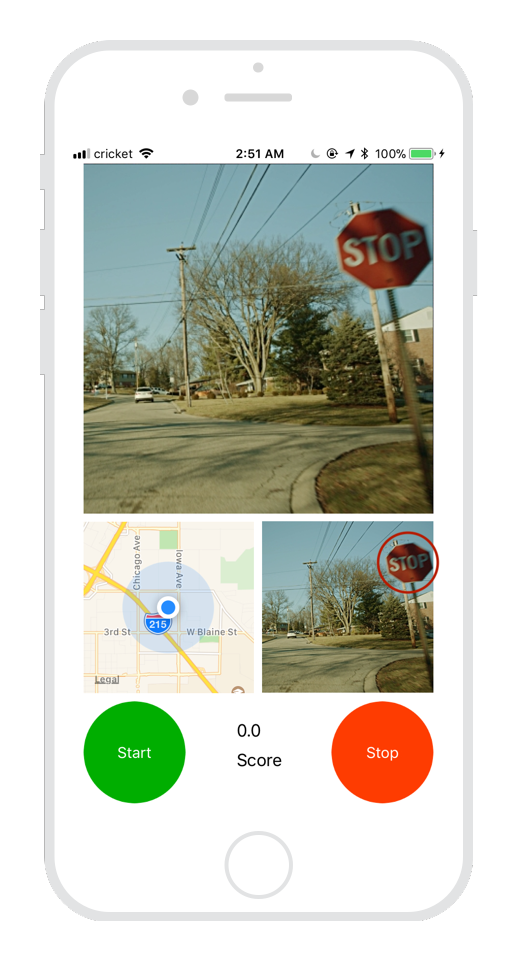
\includegraphics[width=0.6\linewidth]{iOS_design.png}
    \caption{iOS app design}
    \label{fig:fig_1}
  \end{minipage}
\end{figure}

\subsection{Convolutional Neural Network Model}

\subsubsection{Pre-processing}
Here we are using two kinds of datasets:GTSRB and LISA dataset. GTSRB contains 43 kinds of different traffic signs in Germany with 39209 images in the set; LISA, on the other hand, contains 47 kinds of different US traffic signs with 7855 annotations on 6610 frames and 6 super-classes of traffic lights with total 43007 frames and 113888 annotations.Specifically, the images in LISA  were taken in South California, which is more close to our proposed scenario.

The training set would first be pre-processed with normalizing, centering and histogram equalizing to help accelerating the train process on the later section. In addition, augmentation can be applied on them. By using rotation, mirroring and flipping etc., to mimic more possibilities in the real world cases. And the the input image would be separated into training set,validating  and testing set. The example of the common type of sign images in the LISA dataset is shown in Figure 4:

\begin{figure}[hb]
\centering
  \begin{minipage}{.4\textwidth}
    \centering
    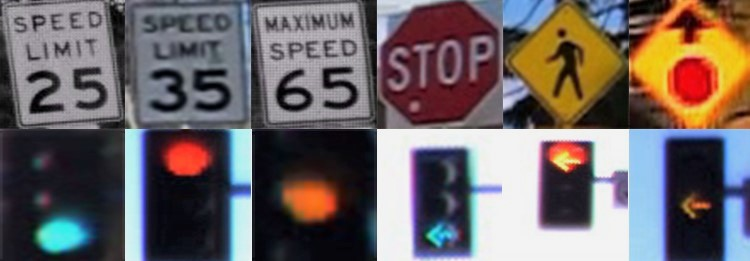
\includegraphics[width=0.8\linewidth]{dataset3.jpg}
    \caption{Example of dataset}
    \label{fig:fig_1}
  \end{minipage}
\end{figure}

\subsubsection{Model Architecture}
In order to do the recognition in our system, we construct a 6-layers CNN network. The model architecture is shown in Figure 5. Each convolutional block contains 2 convolutional layers with the same number of kernel and input/output nodes. Additionally, each block would also followed by a max pooling layer and a drop-out layer. The features extracted by the previous mentioned layer would then be feed to a fully-connected later with dropout. Finally,the softmax layer would aggregate the result and output the probabilities of the input image with regard to each class.

\begin{figure}[H]
\centering
  \begin{minipage}{.5\textwidth}
    \centering
    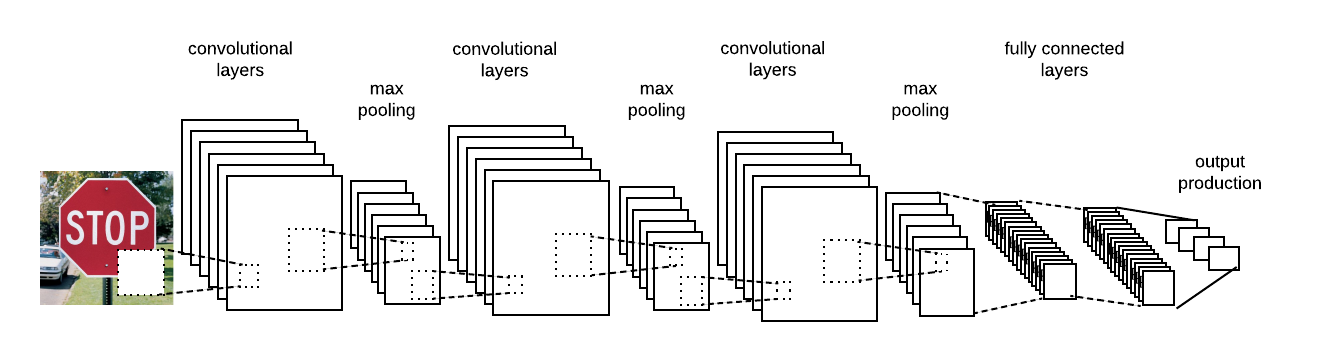
\includegraphics[width=0.8\linewidth]{convolutional_layer.png}
    \caption{CNN architecture}
    \label{fig:fig_1}
  \end{minipage}
\end{figure}

\begin{figure}[hb]
\centering
  \begin{minipage}{.4\textwidth}
    \centering
    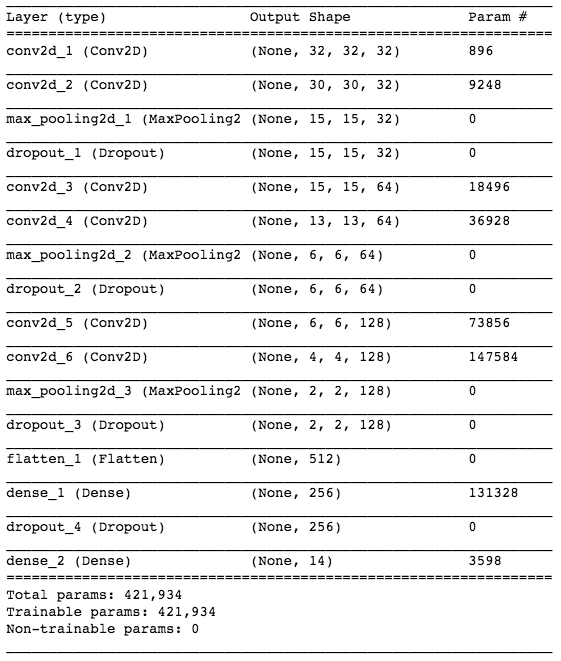
\includegraphics[width=0.8\linewidth]{archi_param.png}
    \caption{CNN layer detail with parameters}
    \label{fig:fig_1}
  \end{minipage}
\end{figure}


\subsection{Cloud Instance Implementation}

We build a computation instance in google cloud with Nvidia P100 GPU.In order to choose the highest performance one to do the comparison, we make some evaluation about different kinds of instance. 

As mentioned above, we use CNN model to recognize traffic signs and traffic lights For CNN model, it can be run either on CPU or GPU.However, we run it on GPU to make it faster. When talking about GPU, it is specifically designed to accelerate the creation of images in a frame buffer intended for output. In order to do this efficiently, GPU needs to have strong ability on computing of the position of geometry points and color. Most of these computations involve vector and matrix operation which are widely used in deep learning model. What is more important, by using GPU, we can do the computation on a large amount of data in higher parallelism. Those are in a nutshell why people use GPU instead of CPU for training a deep learning model. 

According to official references, Google cloud provides three different available GPU models now. They are Nvidia Tesla V100, Nvidia Tesla P100 and Nvidia Tesla K80 respective.However, the Nvidia V100 is for google cloud beta users only. Therefore, we would only do evaluation between Nvidia P100 and Nvidia K80.

% The parameters of different kind models are shown below:

% \begin{figure}[hb]
% \centering
%   \begin{minipage}{.4\textwidth}
%     \centering
%     \includegraphics[width=1.0\linewidth]{gpu.jpg}
%     \caption{cloud instances gpu paramrters}
%     \label{fig:fig_1}
%   \end{minipage}
% \end{figure}

% In our project, we are going to choose the generally available GPUs in Google cloud which are NVIDIA Tesla P100 and NVIDIA Tesla K80 instead of using Nivdia V100 which is only for Google cloud beta users. 

Firstly, we show the key hardware difference between Nvidia P100 and Nvidia K80 

\begin{figure}[H]
\centering
  \begin{minipage}{.4\textwidth}
    \centering
    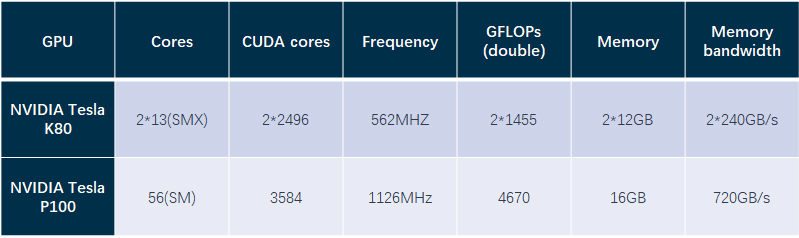
\includegraphics[width=1.0\linewidth]{hardware_parameter.jpg}
    \caption{cloud instances gpu parameters}
    \label{fig:fig_1}
  \end{minipage}
\end{figure}

In the following part, we are going to focus on memory bandwidth and processing power, which are key characteristics of GPU related to machine learning. Besides, we would show the performance of various benchmarks running on different kinds of GPU to verify our evaluation. 

\subsubsection{Memory Bandwidth}
Memory bandwidth would be the most important performance metric while running machine learning model on GPU. It shows the ability of GPU to handle large amount of data. The memory bandwidth of different GPU are shown in table 1:

\begin{table}[htbp]
\caption{Processing power}
\begin{center}
\begin{tabular}{|c|c|}
\hline
\textbf{GPU} & \textbf{\textit{Memory bandwidth}}\\
\hline
Nvidia Tesla K80 & 240GB/s per core \\
\hline
Nvidia Tesla P100 & 720GB/s per core\\
\hline
\end{tabular}
\label{tab1}
\end{center}
\end{table}


From the table, we can get that P100 's memory bandwidth is $3 \times$ bigger than K80 per core. 

\subsubsection{Processing Power}
Processing power is also a key characteristic we need to focus on while choosing our GPU. It indicates the highest speed GPU can achieve to crunch data. We use the number of CUDA cores multiplied by the frequency of the core to present it.
$$Processing \ power = Number \ of \ CUDA \ cores \times frequency $$

The result is shown in table 2:

\begin{table}[htbp]
\caption{Processing power}
\begin{center}
\begin{tabular}{|c|c|c|c|}
\hline
\textbf{GPU} & \textbf{\textit{CUDA cores}}& \textbf{\textit{frequency}}& \textbf{\textit{Processing power}} \\
\hline
Nvidia Tesla K80 & 2496(per core)& 562MHz & 1402752 \\
\hline
Nvidia Tesla P100 & 3584(per core)& 1126MHz & 4035584 \\
\hline
\end{tabular}
\label{tab2}
\end{center}
\end{table}

\subsubsection{Benchmark Result}

Our machine learning code is built based on Tensorflow, therefore we get some evaluation for the influence of different kinds of GPU in various benchmarks, which include Tensorflow. Those benchmark information are gotten from microway.com[5]

The benchmarks result are shown below:
\begin{figure}[H]
\centering
  \begin{minipage}{.4\textwidth}
    \centering
    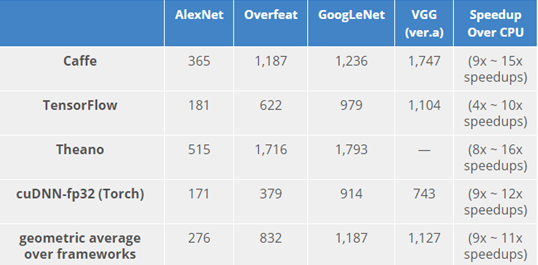
\includegraphics[width=1.0\linewidth]{k80_benchmark.jpg}
    \caption{K80 benchmark result}
    \label{fig:fig_1}
  \end{minipage}
\end{figure}

\begin{figure}[H]
\centering
  \begin{minipage}{.4\textwidth}
    \centering
    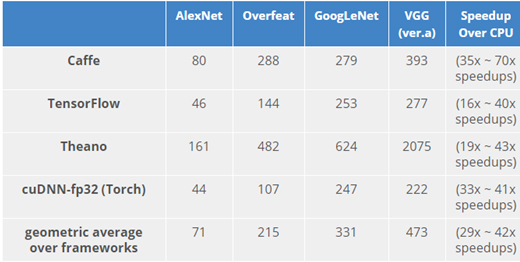
\includegraphics[width=1.0\linewidth]{P100_benchmark.jpg}
    \caption{P100 benchmark result}
    \label{fig:fig_1}
  \end{minipage}
\end{figure}

\begin{figure}[H]
\centering
  \begin{minipage}{.4\textwidth}
    \centering
    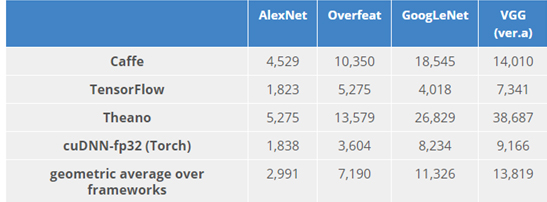
\includegraphics[width=1.0\linewidth]{cpu_only.jpg}
    \caption{CPU only benchmark result}
    \label{fig:fig_1}
  \end{minipage}
\end{figure}

From the experiment, we can get that the speed up over CPU of Nvidia P100 is $4 \times$ higher than speed up over CPU of Nvidia K80 on Tensorflow. 

The comparison above shows the Nvidia Tesla P100 GPU is outperform than Nvidia Tesla K80 from every aspects. 

\section{Evaluation}

\subsection{Experimental setup}

The parameters of platforms we would implement our system on to do the evaluation is shown as follows: 

% \begin{longtable}
% \caption{platforms setup}
% \begin{center}
% \begin{tabular}{|c|c|c|c|}
% \hline
% \textbf{} & \textbf{\textit{mobile device}}& \textbf{\textit{google cloud}}& \textbf{\textit{terminal machine}} \\
% \hline
% CPU & 1.85GHz-dual core-64-bit-ARMv8-A&2.2GHz Intel Xeon E5 v4(Boardwell)& I5 6400 \\
% \hline
% Nvidia Tesla P100 & 3584(per core)& 1126MHz & 4035584 \\
% \hline
% \end{tabular}
% \label{tab1}
% \end{center}
% \end{longtable}


\subsection{Experiment Evaluation}

\subsubsection{CNN model evaluation}

\begin{table}[H]
\caption{CNN model test result}
\begin{center}
\begin{tabular}{|c|c|c|}
\hline
\textbf{Dataset} & \textbf{\textit{No. of classes}}& \textbf{\textit{Test accuracy}} \\
\hline
GTSRB & 43 & 96.4\% \\
\hline
LISA Traffic Sign & 14 & 99.8\% \\
\hline
LISA Traffic Light& 6 & 99.5\% \\
\hline
\end{tabular}
\label{tab3}
\end{center}
\end{table}

\begin{figure}[H]
\centering
  \begin{minipage}{.3\textwidth}
    \centering
    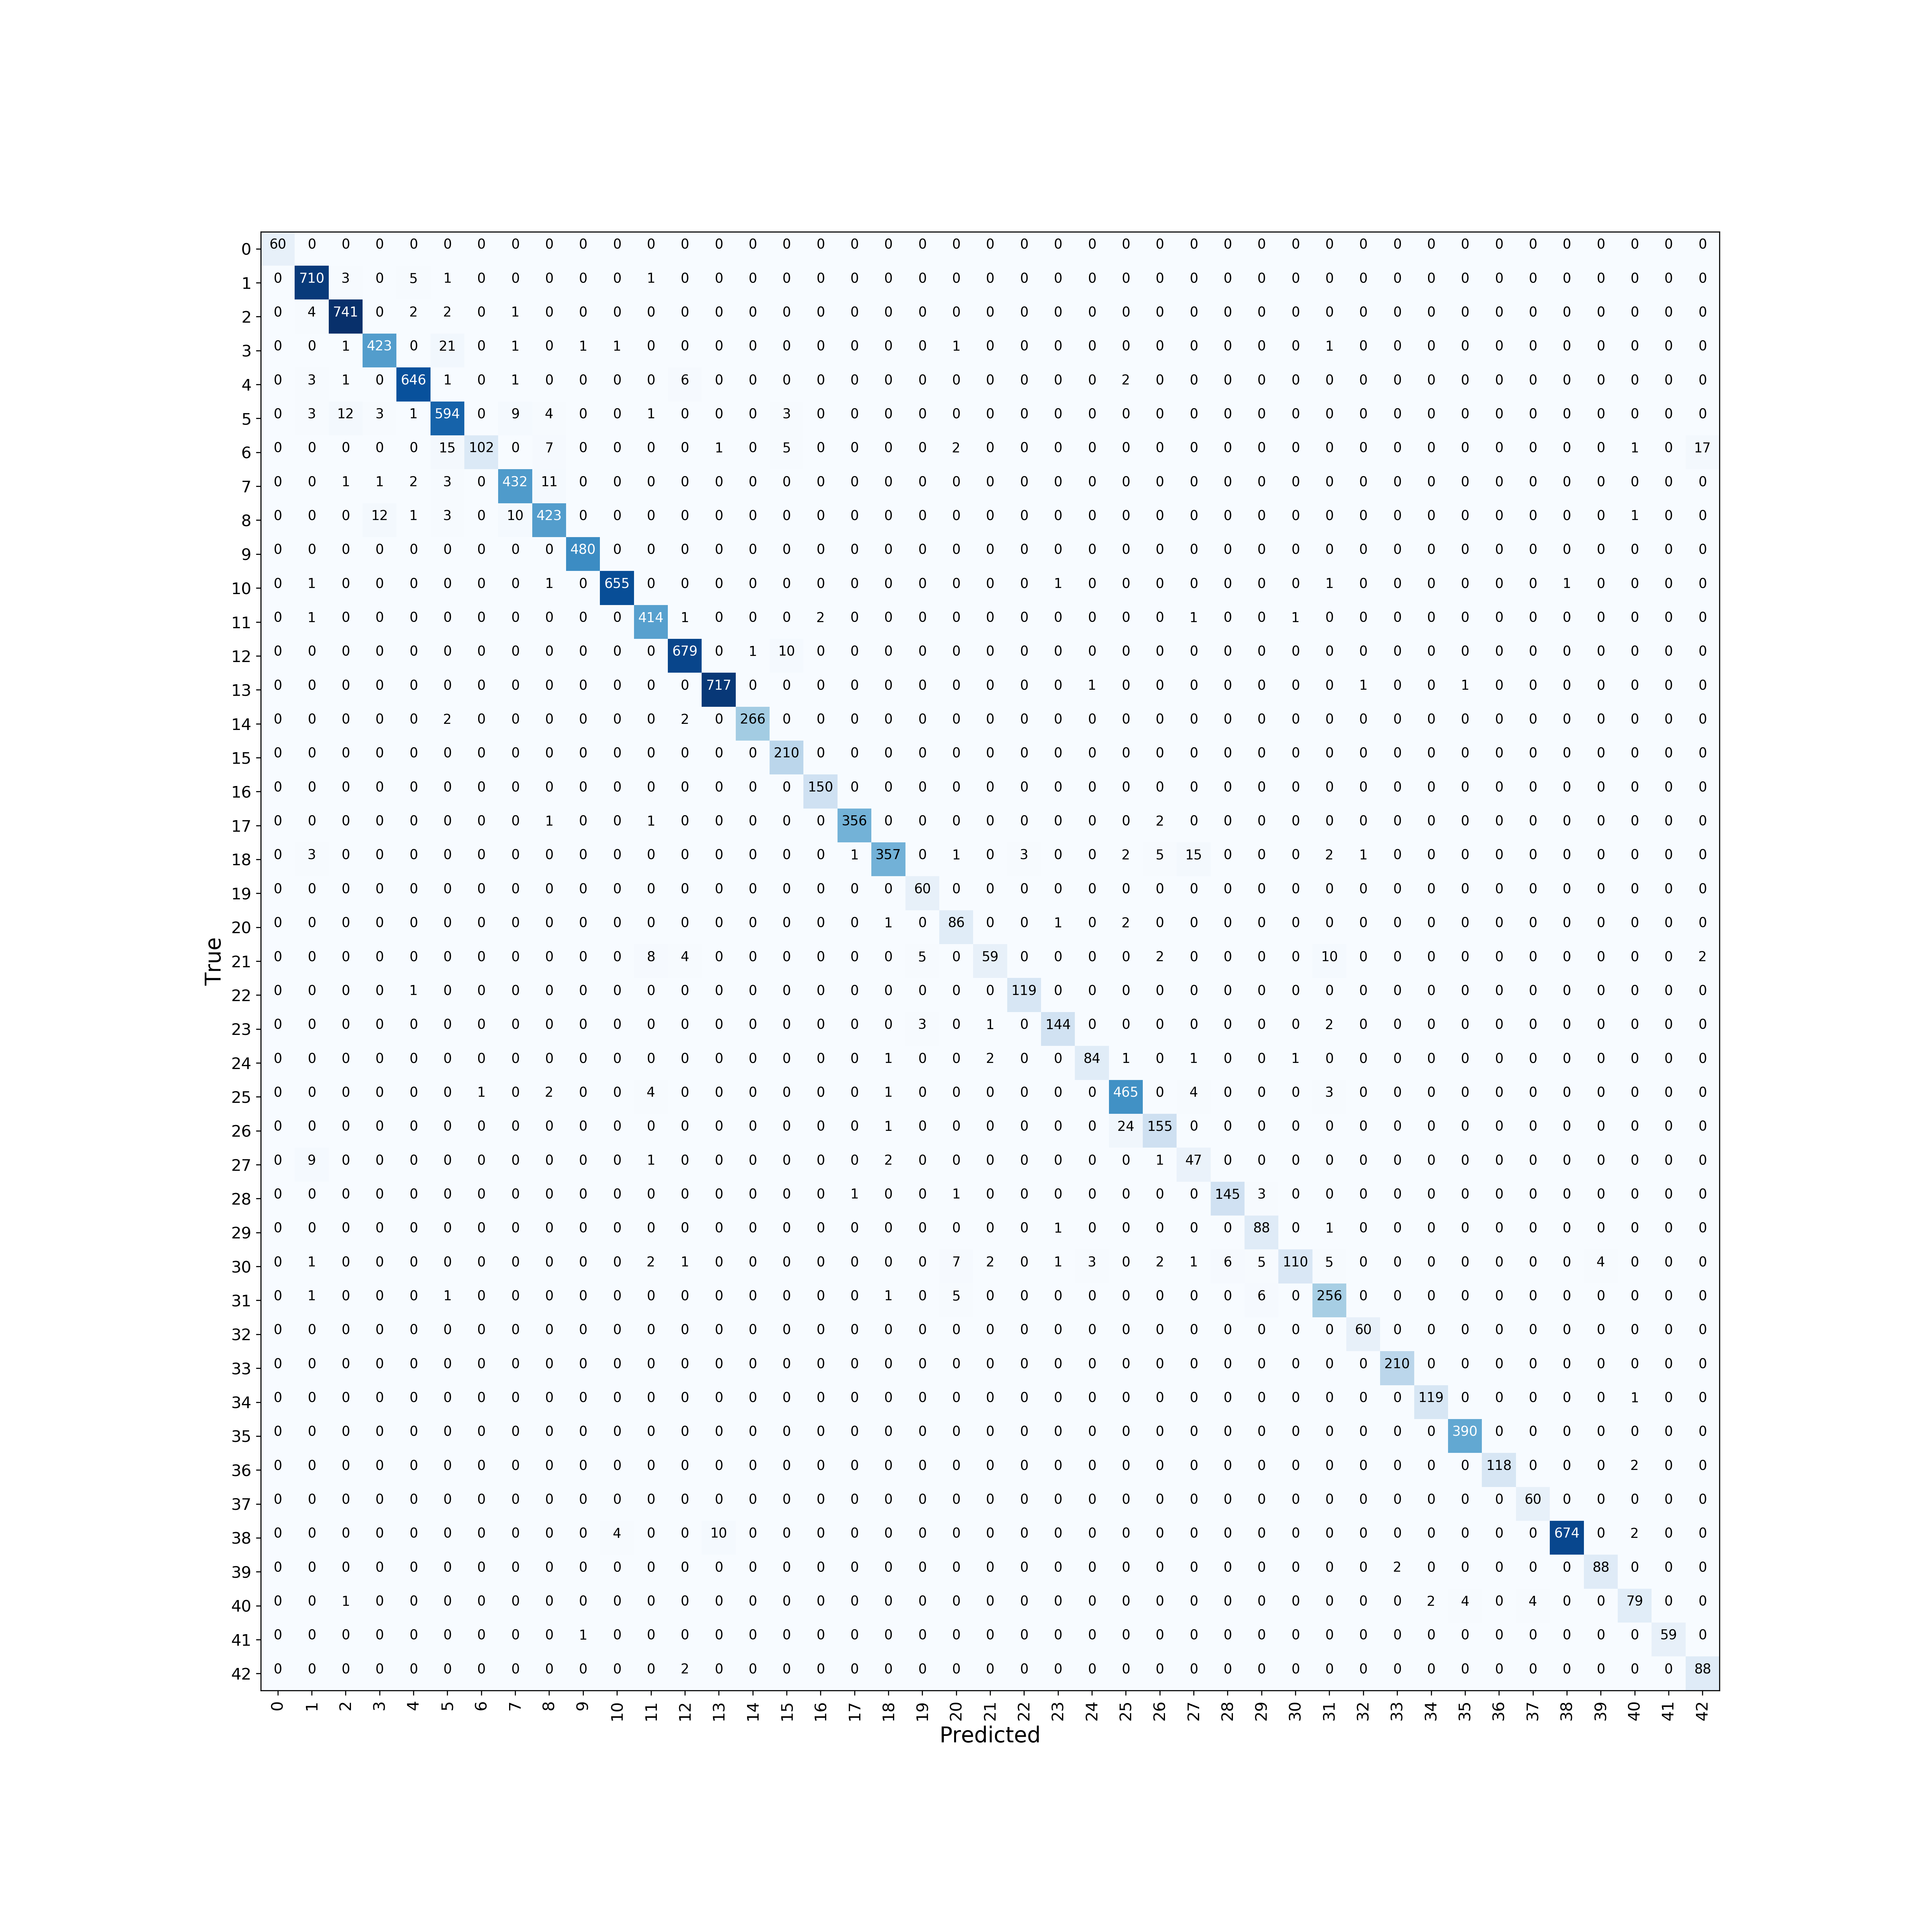
\includegraphics[width=1.0\linewidth]{confusion_matrix_f.png}
    \caption{Testing confusion matrix with GTSRB}
    \label{fig:fig_1}
  \end{minipage}
\end{figure}
\begin{figure}[H]
\centering
  \begin{minipage}{.3\textwidth}
    \centering
    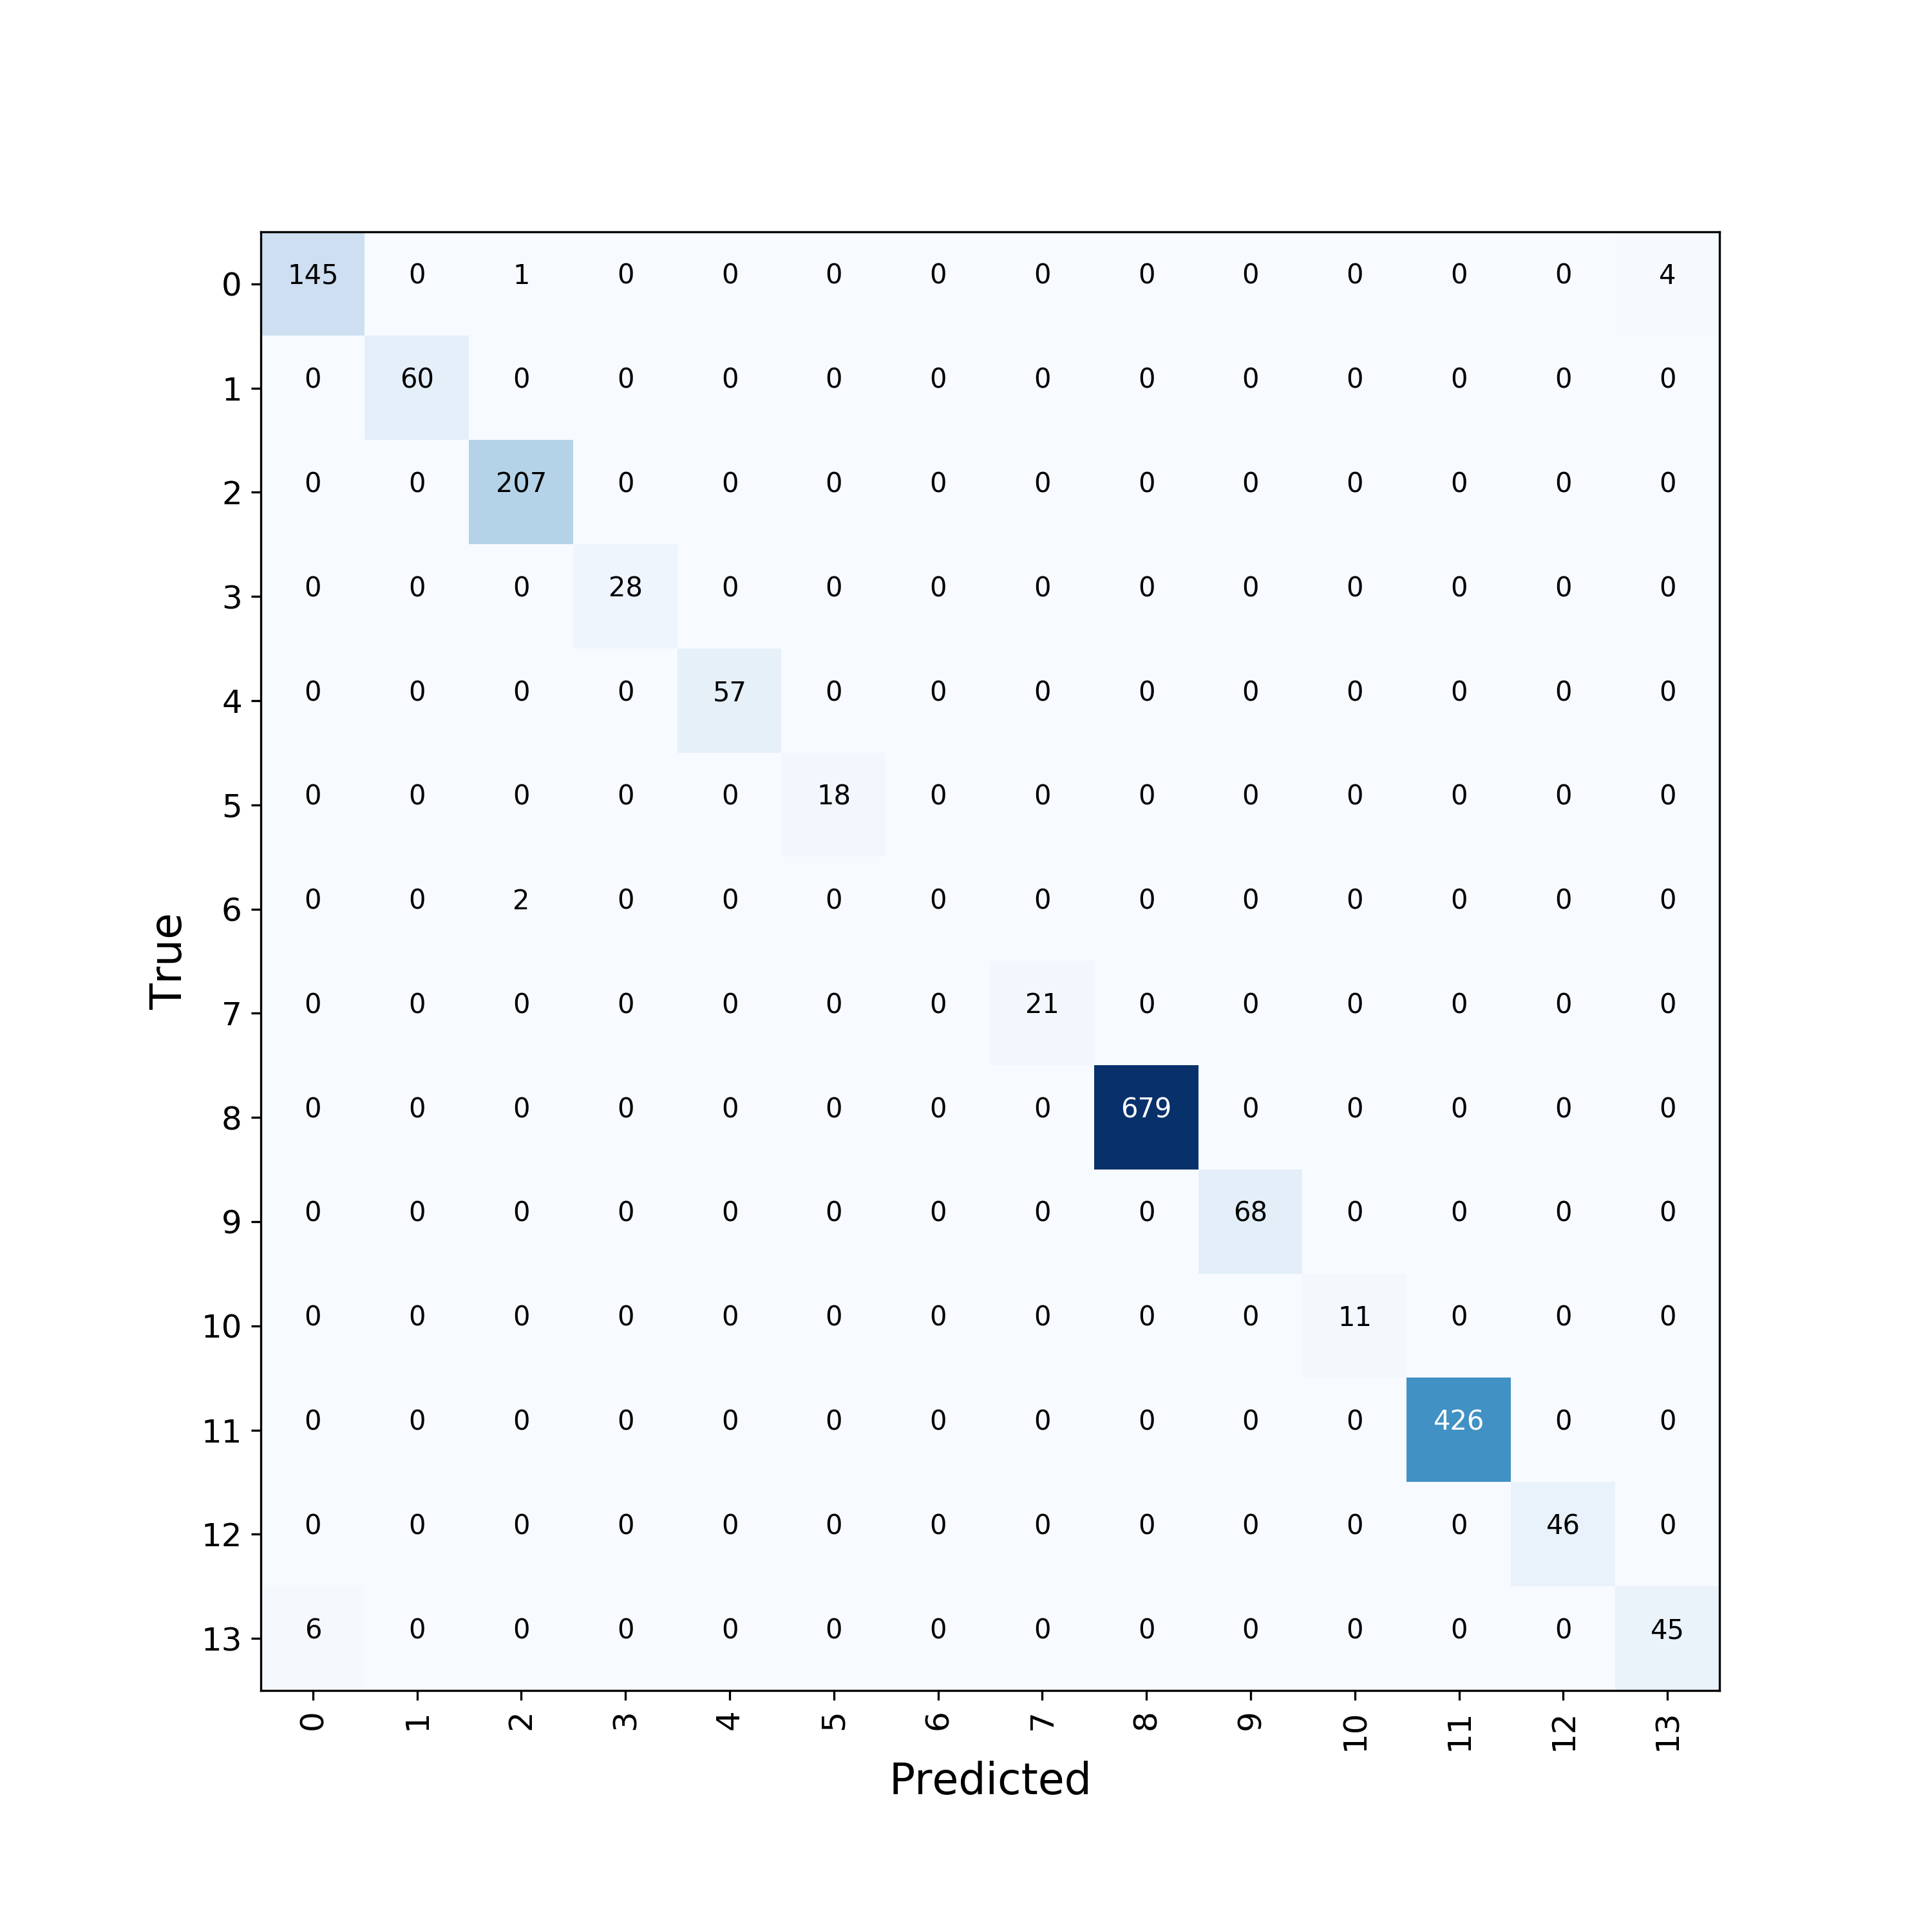
\includegraphics[width=1.0\linewidth]{confusion_matrix.png}
    \caption{Testing confusion matrix with LISA traffic sign}
    \label{fig:fig_1}
  \end{minipage}
\end{figure}
\begin{figure}[H]
\centering
  \begin{minipage}{.3\textwidth}
    \centering
    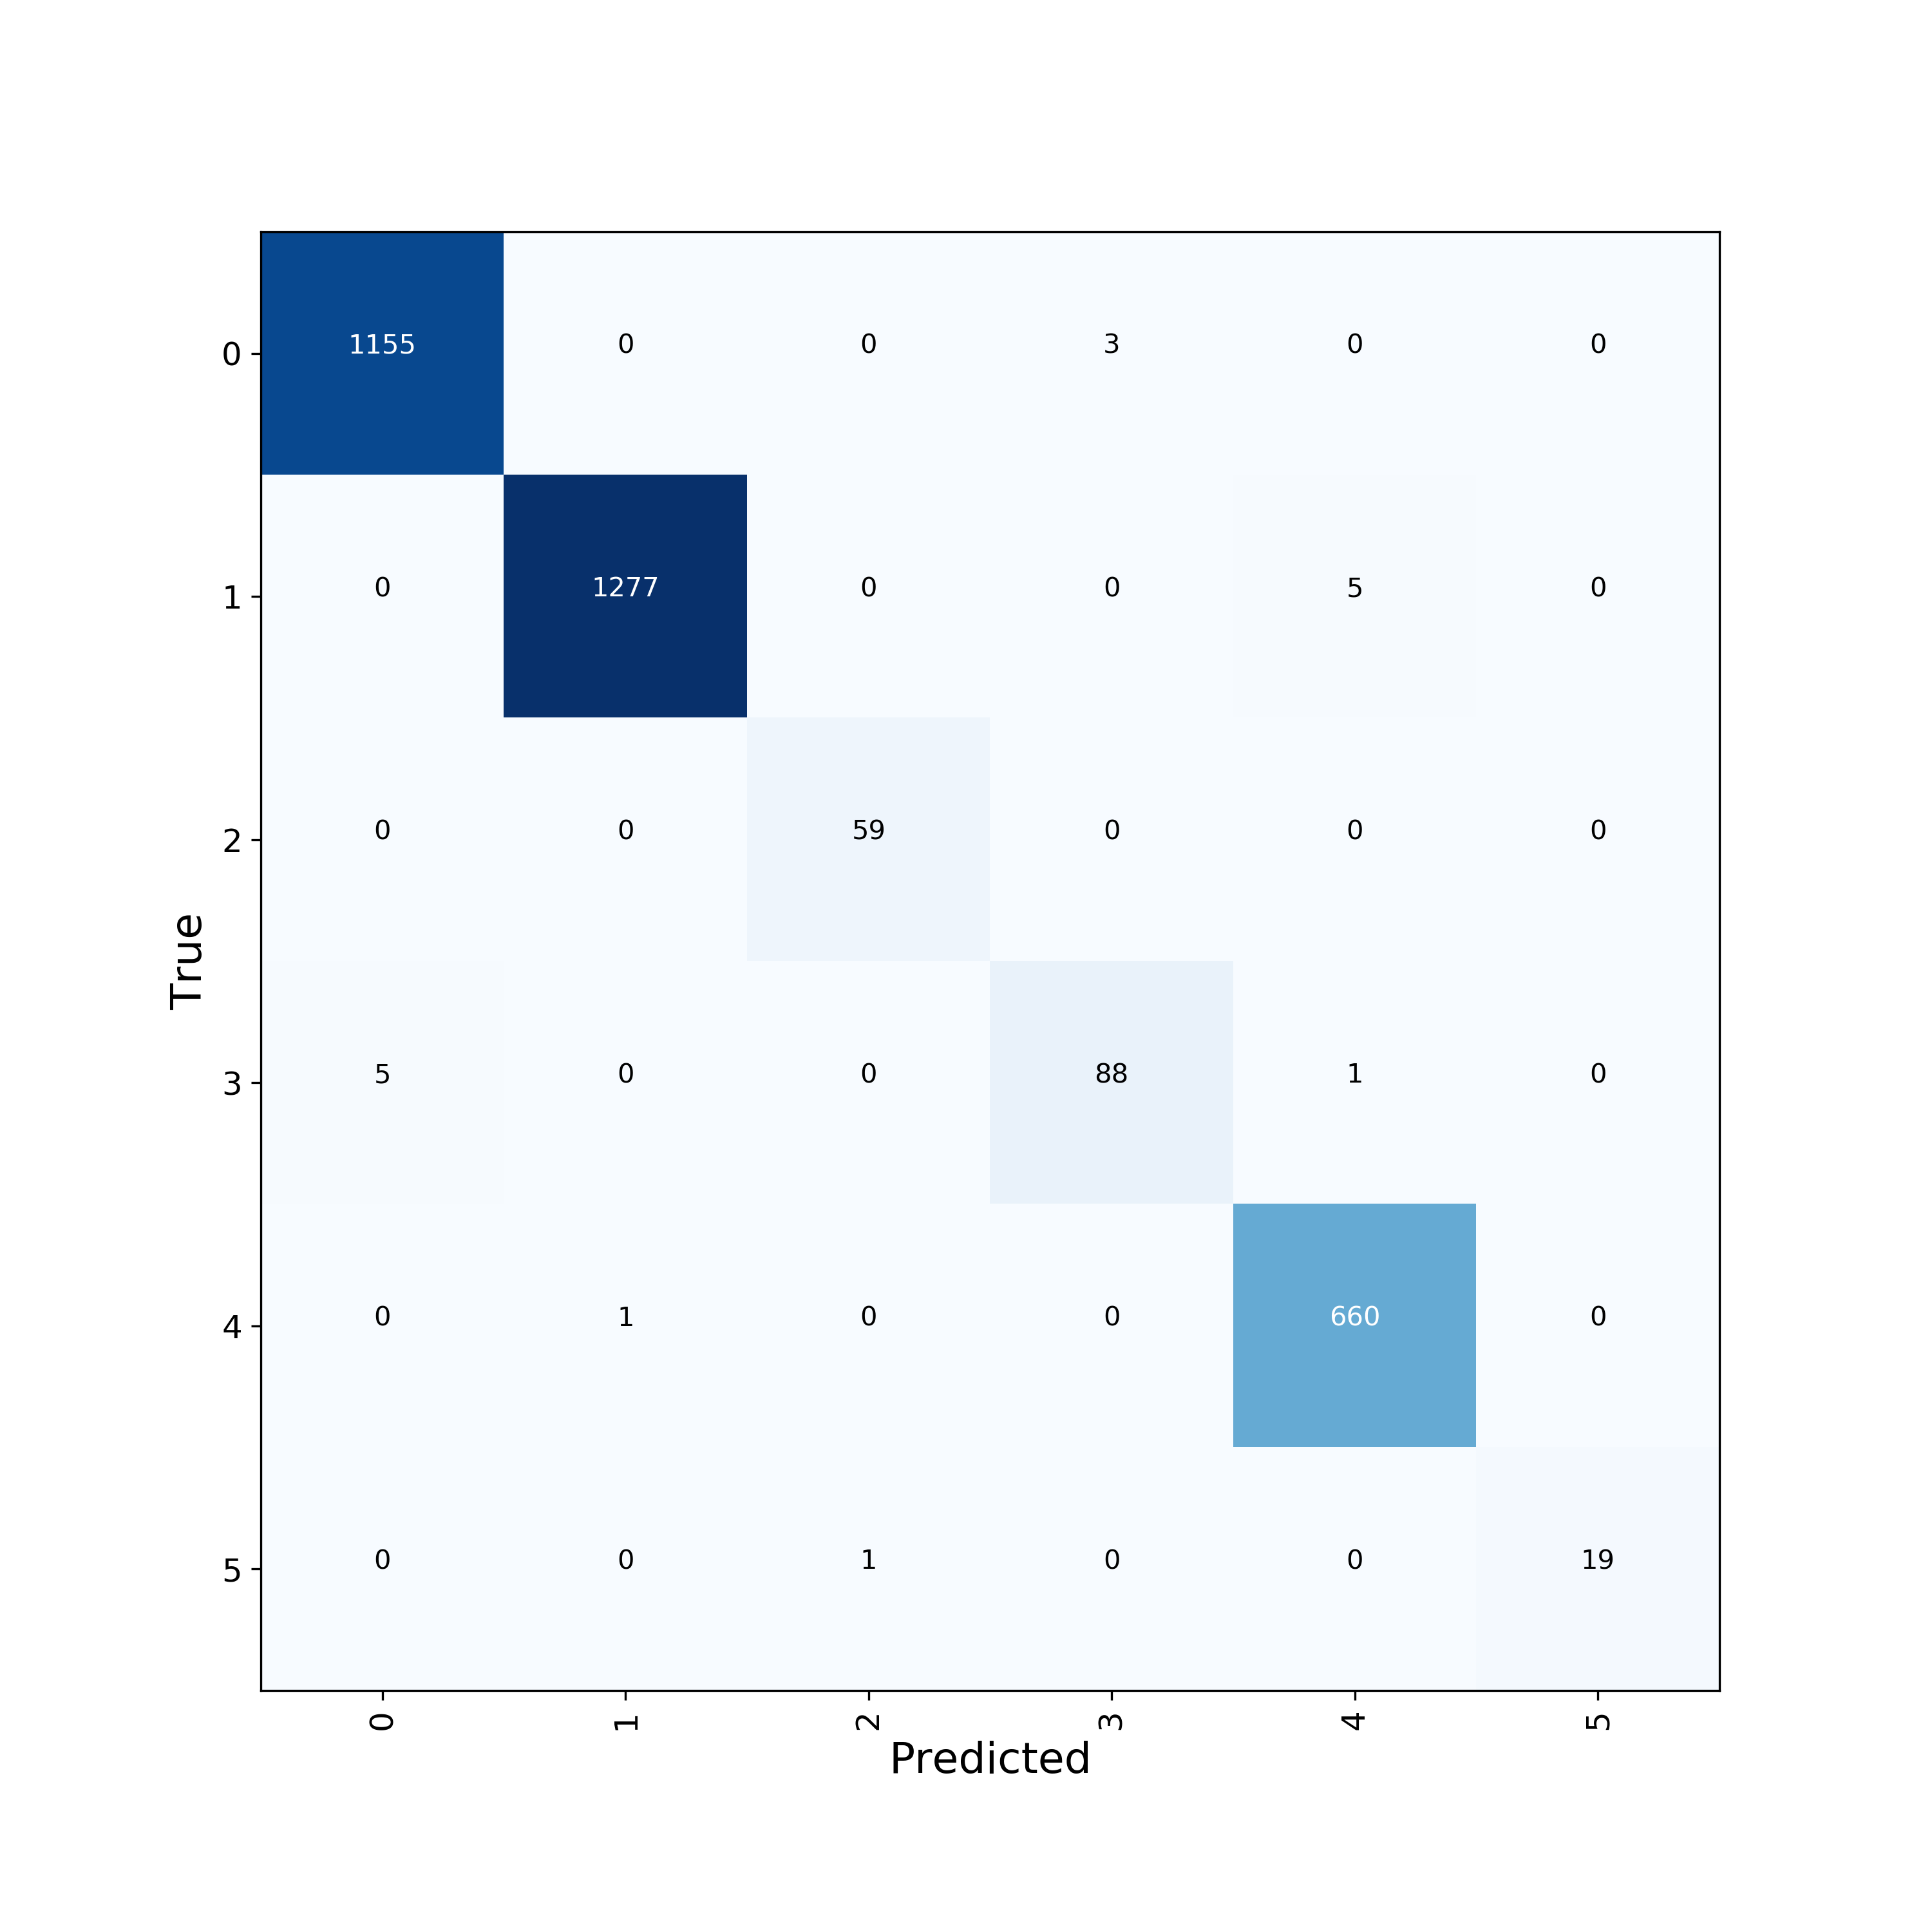
\includegraphics[width=1.0\linewidth]{confusion_matrix_traffic_light.png}
    \caption{Testing confusion matrix with LISA traffic light}
    \label{fig:fig_1}
  \end{minipage}
\end{figure}

\begin{thebibliography}{00}
\bibitem{b1} G. Eason, B. Noble, and I. N. Sneddon, ``On certain integrals of Lipschitz-Hankel type involving products of Bessel functions,'' Phil. Trans. Roy. Soc. London, vol. A247, pp. 529--551, April 1955.
\bibitem{b2} J. Clerk Maxwell, A Treatise on Electricity and Magnetism, 3rd ed., vol. 2. Oxford: Clarendon, 1892, pp.68--73.
\bibitem{b3} I. S. Jacobs and C. P. Bean, ``Fine particles, thin films and exchange anisotropy,'' in Magnetism, vol. III, G. T. Rado and H. Suhl, Eds. New York: Academic, 1963, pp. 271--350.
\bibitem{b4} K. Elissa, ``Title of paper if known,'' unpublished.
\bibitem{b5} R. Nicole, ``Title of paper with only first word capitalized,'' J. Name Stand. Abbrev., in press.
\bibitem{b6} Y. Yorozu, M. Hirano, K. Oka, and Y. Tagawa, ``Electron spectroscopy studies on magneto-optical media and plastic substrate interface,'' IEEE Transl. J. Magn. Japan, vol. 2, pp. 740--741, August 1987 [Digests 9th Annual Conf. Magnetics Japan, p. 301, 1982].
\bibitem{b7} M. Young, The Technical Writer's Handbook. Mill Valley, CA: University Science, 1989.
\end{thebibliography}
\vspace{12pt}
\color{red}
IEEE conference templates contain guidance text for composing and formatting conference papers. Please ensure that all template text is removed from your conference paper prior to submission to the conference. Failure to remove the template text from your paper may result in your paper not being published.

\end{document}
